\documentclass[12pt,a4paper]{article}

% ---- Codificación y lengua ----
\usepackage[utf8]{inputenc}
\usepackage[T1]{fontenc}
\usepackage[provide=*,spanish]{babel}

% ---- Márgenes ----
\usepackage[top=2.5cm, bottom=2.5cm, left=3cm, right=2.5cm]{geometry}

% ---- Tipografía ----
\usepackage{lmodern}
\usepackage{microtype}

% ---- Matemáticas ----
\usepackage{amsmath}
\usepackage{amssymb}

% ---- Colores ----
\usepackage[dvipsnames,svgnames,table]{xcolor}
\definecolor{azulAS}{RGB}{30,90,160}
\definecolor{verdePos}{RGB}{46,125,50}
\definecolor{rojoNeg}{RGB}{183,28,28}
\definecolor{grisCelda}{RGB}{240,245,250}
\definecolor{naranjaAdv}{RGB}{217,119,6}
\definecolor{moradoNMF}{RGB}{123,31,162}

% ---- Gráficos y figuras ----
\usepackage{graphicx}
\usepackage{float}
\usepackage{caption}
\captionsetup{font=small, labelfont=bf}

% ---- TikZ para diagramas ----
\usepackage{tikz}
\usetikzlibrary{shapes.geometric, arrows.meta, positioning, shapes, calc, fit, backgrounds}

% ---- Tablas ----
\usepackage{booktabs}
\usepackage{longtable}
\usepackage{array}
\usepackage{tabularx}
\usepackage{colortbl}
\newcolumntype{C}{>{\centering\arraybackslash}X}

% ---- Código fuente ----
\usepackage{listings}
\lstset{
  basicstyle=\ttfamily\footnotesize,
  backgroundcolor=\color{grisCelda},
  frame=single,
  breaklines=true,
  captionpos=b,
  keywordstyle=\color{azulAS}\bfseries,
  commentstyle=\color{verdePos},
  stringstyle=\color{rojoNeg},
  language=Python,
  numbers=left,
  numberstyle=\tiny\color{gray},
  numbersep=5pt,
  showstringspaces=false,
  tabsize=2,
  extendedchars=true,
  inputencoding=utf8,
  literate=
    {á}{{\'a}}1 {é}{{\'e}}1 {í}{{\'i}}1 {ó}{{\'o}}1 {ú}{{\'u}}1
    {Á}{{\'A}}1 {É}{{\'E}}1 {Í}{{\'I}}1 {Ó}{{\'O}}1 {Ú}{{\'U}}1
    {ñ}{{\~n}}1 {Ñ}{{\~N}}1
    {ü}{{\"u}}1 {¿}{{?`}}1 {¡}{{!`}}1
}

% ---- Hipervínculos ----
\usepackage[colorlinks=true, linkcolor=azulAS, citecolor=verdePos,
            urlcolor=azulAS, bookmarks=true]{hyperref}

% ---- Encabezados ----
\usepackage{fancyhdr}
\setlength{\headheight}{14pt}
\pagestyle{fancy}
\fancyhf{}
\fancyhead[L]{\small Análisis de Congestión Vial --- La Paz y El Alto}
\fancyhead[R]{\small \thepage}
\renewcommand{\headrulewidth}{0.4pt}

\emergencystretch=3em

% ---- Espaciado ----
\usepackage{setspace}
\onehalfspacing

% ---- Secciones con color ----
\usepackage{titlesec}
\titleformat{\section}{\large\bfseries\color{azulAS}}{\thesection.}{0.5em}{}[\titlerule]
\titleformat{\subsection}{\normalsize\bfseries\color{azulAS}}{\thesubsection.}{0.5em}{}
\titleformat{\subsubsection}{\normalsize\itshape\color{azulAS}}{\thesubsubsection.}{0.5em}{}

% ---- Enumeraciones ----
\usepackage{enumitem}

% ---- Cajas de información ----
\newsavebox{\advboxcontent}
\newenvironment{advbox}{%
  \par\addvspace{6pt}%
  \begin{lrbox}{\advboxcontent}%
  \begin{minipage}{\dimexpr\linewidth-16pt}%
  \small\color{naranjaAdv!80!black}%
}{%
  \end{minipage}%
  \end{lrbox}%
  \noindent\colorbox{yellow!12}{\usebox{\advboxcontent}}%
  \par\addvspace{6pt}%
}

\newsavebox{\conceptboxcontent}
\newenvironment{conceptbox}[1]{%
  \par\addvspace{6pt}%
  \begin{lrbox}{\conceptboxcontent}%
  \begin{minipage}{\dimexpr\linewidth-16pt}%
  \small\color{azulAS!80!black}%
  \textbf{#1}\par\smallskip%
}{%
  \end{minipage}%
  \end{lrbox}%
  \noindent\colorbox{azulAS!7}{\usebox{\conceptboxcontent}}%
  \par\addvspace{6pt}%
}

\begin{document}

%=================================================================
% CARÁTULA
%=================================================================
\begin{titlepage}
  \thispagestyle{empty}
  \singlespacing
  \centering

  \vspace*{0.5cm}

  {\Large\bfseries Universidad Mayor de San Andrés}\\[0.3em]
  {\normalsize Facultad de Ciencias Puras y Naturales}\\[0.15em]
  {\normalsize Carrera de Informática}

  \vspace{0.5cm}

  
\includegraphics[width=2.8cm]{img/Logo_Umsa.png}

  \vspace{0.6cm}

  {\color{azulAS}\rule{\linewidth}{1.5pt}}
  \vspace{0.35cm}

  {\LARGE\bfseries Tráfico Inteligente}\\[0.35em]
  {\large Análisis no supervisado de la congestión vial\\[0.15em]
   en La Paz y El Alto, Bolivia\\[0.15em]
   mediante Aprendizaje Automático No Supervisado}

  \vspace{0.35cm}
  {\color{azulAS}\rule{\linewidth}{1.5pt}}

  \vspace{0.7cm}

  {\large Maximiliano Gómez Mallo}\\[0.15em]
  {\normalsize 14480221}

  \vspace{0.7cm}

  \begin{tabular}{ll}
    \textbf{Materia:}  & Machine Learning               \\[0.25em]
    \textbf{Docente:}  & Menfy Morales Rios             \\[0.25em]
    \textbf{Fecha:}    & La Paz, Bolivia --- Mayo 2026  \\
  \end{tabular}

\end{titlepage}

%=================================================================
% TABLA DE CONTENIDOS
%=================================================================
\newpage
\tableofcontents
\newpage

%=================================================================
\section{Introducción}
%=================================================================

La ciudad de La Paz y su vecina El Alto conforman una de las conurbaciones
más complejas de América del Sur desde el punto de vista vial.
La Paz descansa en una hoya montañosa a unos 3\,600 m.s.n.m., mientras que
El Alto se extiende en el altiplano a 4\,100 m.s.n.m.;
ambas ciudades están conectadas por apenas unas pocas autopistas de alta
pendiente, lo que convierte cualquier incidente en una cascada de congestión
que puede paralizar barrios enteros durante horas.

\medskip

\textbf{Objetivo del proyecto.}
Clasificar automáticamente segmentos de carretera según su patrón de
congestión \emph{sin utilizar etiquetas previas} —es decir, sin que nadie
haya definido de antemano qué significa ``alta congestión'' o ``zona
tranquila''.
Para ello aplicamos un conjunto de algoritmos de \textbf{aprendizaje no
supervisado}: reducción de dimensionalidad (PCA, UMAP), clustering espacial
(DBSCAN) y temporal (K-Means), y síntesis de datos faltantes (NMF + PCHIP).

\medskip

El resultado final es un \textbf{dashboard interactivo} que permite a
cualquier usuario explorar el comportamiento del tráfico hora a hora, día
a día, y comparar ambas ciudades de forma visual e intuitiva.

\subsection{¿Por qué aprendizaje no supervisado?}

En el aprendizaje supervisado, alguien debe etiquetar los datos previamente:
``esta calle es alta congestión'', ``esta otra es tranquila''.
Esto requiere expertos, tiempo y dinero.

En el aprendizaje \textbf{no supervisado}, el algoritmo descubre la
estructura por sí mismo, preguntando: \textit{¿qué segmentos se parecen entre
sí?} Esta pregunta es mucho más poderosa cuando los datos son complejos:
en lugar de clasificar calles en dos categorías rígidas, el modelo puede
descubrir grupos más sutiles que un humano nunca habría definido a priori.

%=================================================================
\section{Adquisición de datos}
%=================================================================

\subsection{Medición de congestión: el jam factor}

Para medir la congestión usamos la \textit{Distance Matrix API} de Google,
que devuelve el tiempo de viaje entre pares de puntos con y sin tráfico.
De estos dos valores calculamos el \textbf{jam factor}:

\begin{equation}
  \text{jam\_factor} = \frac{\text{duración con tráfico}}{\text{duración típica}}
  \label{eq:jam}
\end{equation}

\begin{conceptbox}{¿Cómo interpretar el jam factor?}
  Un jam\_factor de $1{,}0$ significa tráfico fluido: el viaje tarda lo esperado.
  Un valor de $2{,}5$ indica que el trayecto toma \textit{2,5 veces} más de lo normal.
  En La Paz, los valores oscilan entre $1{,}0$ (madrugada, calles vacías) y
  $\approx 3{,}5$ (hora pico, centros comerciales).
\end{conceptbox}

\subsection{Red vial: OSMnx}

Para definir \emph{qué} calles consultar, usamos \textbf{OSMnx}, una
librería Python que descarga el grafo vial de OpenStreetMap gratuitamente.
Cada segmento (arista del grafo) tiene coordenadas GPS de inicio y fin,
longitud en metros y tipo de vía.

\medskip

El grafo de La Paz contiene $\approx 37\,100$ segmentos de calle.
Consultar todos excedería el presupuesto de la API, así que
\textbf{muestreamos 250 segmentos por zona} estratificando por tipo de vía
para garantizar que autopistas, avenidas y calles residenciales estén
representadas proporcionalmente.

\begin{figure}[H]
  \centering
  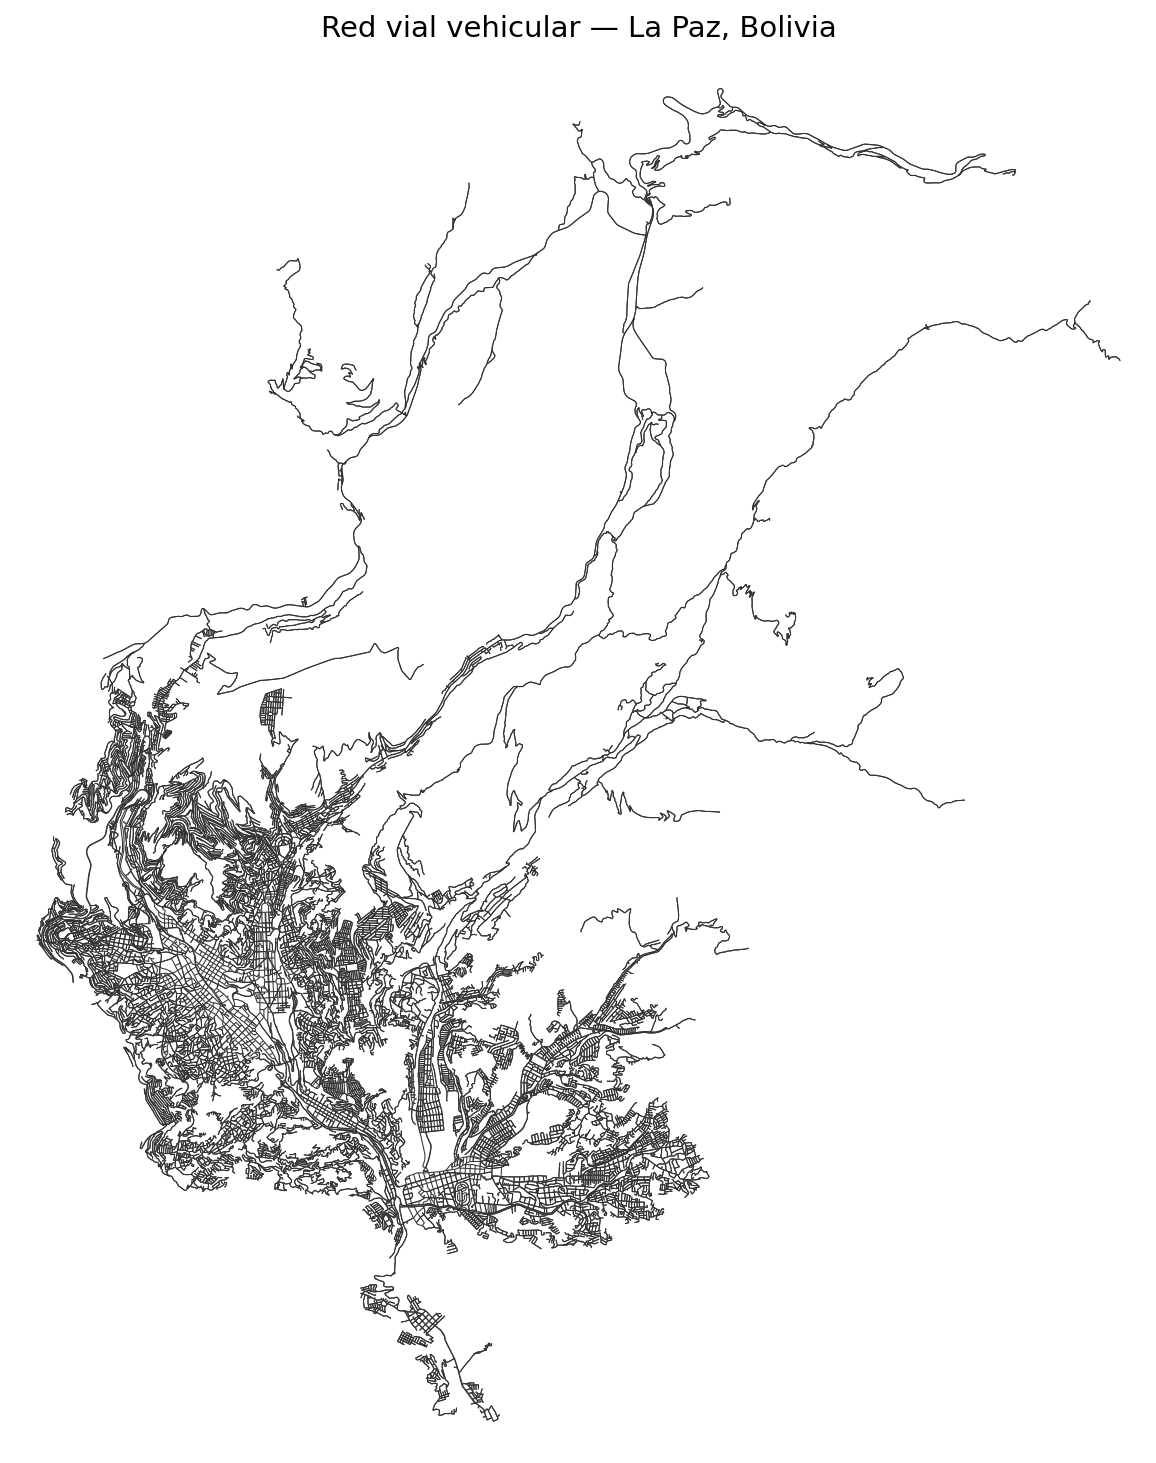
\includegraphics[width=0.82\textwidth]{img/red_vial.png}
  \caption{Red vial completa de La Paz descargada con OSMnx (37\,100 segmentos).
           El grafo captura desde autopistas hasta calles locales.}
  \label{fig:red_vial}
\end{figure}

\begin{lstlisting}[caption={Descarga del grafo vial y muestreo estratificado.}]
import osmnx as ox

G = ox.graph_from_place("La Paz, Bolivia", network_type="drive")
edges = ox.graph_to_gdfs(G, nodes=False)   # 37 100 aristas

# Muestreo estratificado por tipo de via
sample = (
    edges.groupby("highway", group_keys=False)
         .apply(lambda g: g.sample(min(len(g), 30), random_state=42))
)
sample = sample.sample(250, random_state=42).reset_index()
\end{lstlisting}

\subsection{Días y horas recolectados}

Por restricciones de cuota de la API se recolectaron \textbf{4 días} representativos
de la semana: lunes (día laboral típico), miércoles (mitad de semana),
viernes (día laboral con tráfico extra) y sábado (fin de semana).
Para cada día se consultaron las 24 horas, obteniendo un retrato completo
del comportamiento diario.

\begin{figure}[H]
  \centering
  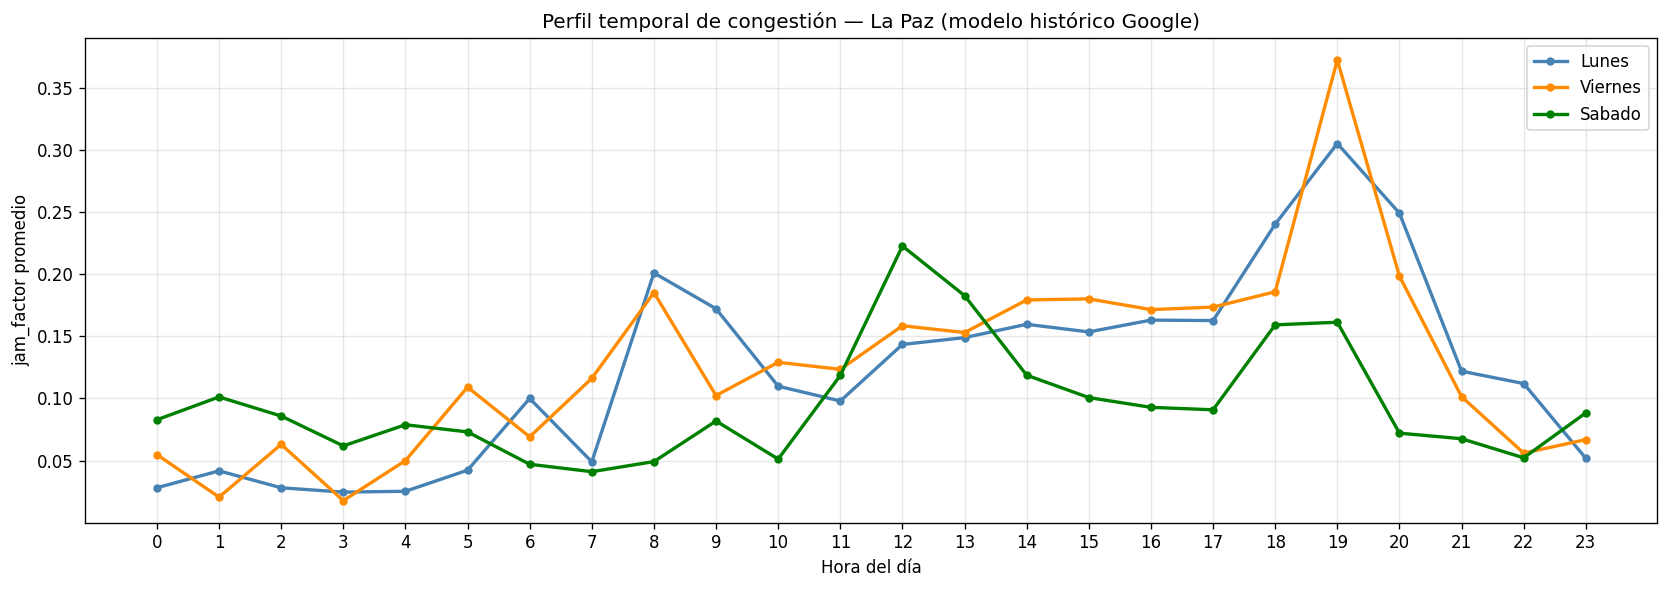
\includegraphics[width=0.90\textwidth]{img/perfiles_raw.png}
  \caption{Perfiles de congestión por hora del día para los distintos días recolectados.
           Se aprecia el pico matutino (7--9 h) y vespertino (17--19 h) característicos
           de La Paz, y el patrón más suave del sábado.}
  \label{fig:perfiles_raw}
\end{figure}

%=================================================================
\section{Construcción de la feature matrix}
%=================================================================

\subsection{Concepto: la tabla de datos}

Antes de aplicar cualquier modelo, necesitamos representar cada segmento
vial como un \textbf{vector numérico}: una lista de números que describa su
comportamiento de tráfico.
A esta tabla de vectores la llamamos \textbf{feature matrix}
(matriz de características).

Cada fila es un segmento; cada columna es el jam\_factor promedio en una
combinación \{día, hora\}:

\begin{equation}
  X \in \mathbb{R}^{250 \times 96}
  \quad\text{donde}\quad
  X_{i,\,d \cdot 24 + h} = \text{jam\_factor del segmento } i
  \text{ el día } d \text{ a las } h\text{ horas}
  \label{eq:fmat}
\end{equation}

Los 96 columnas provienen de $4\,\text{días} \times 24\,\text{h/día}$.

\begin{advbox}
  \textbf{¿Por qué usar las 24 horas y no solo la hora pico?}
  Las horas pico (7--9 h, 17--19 h) capturan el máximo de congestión,
  pero el \emph{patrón completo} del día —cómo sube y baja el tráfico a lo largo
  de las 24 horas— distingue mejor los tipos de calle.
  Una avenida comercial está congestionada también al mediodía; una autopista
  de salida solo en horas pico.
  Al incluir todas las horas, los modelos pueden capturar estas diferencias sutiles.
\end{advbox}

\begin{lstlisting}[caption={Construcción de la feature matrix (script 03).}]
DIAS = ["lunes", "miercoles", "viernes", "sabado"]
mat  = segs.set_index("segment_id").copy()

for dia in DIAS:
    for h in range(24):
        f   = traffic_dir / f"traffic_{dia}_{h:02d}.csv"
        col = f"jam_{dia}_{h:02d}"
        df  = pd.read_csv(f)[["segment_id", "jam_factor"]]
        mat[col] = df.set_index("segment_id")["jam_factor"]

mat = mat.fillna(0.0)   # segmentos sin dato -> fluido (1.0 normalizado)
mat.to_csv(output_csv)
\end{lstlisting}

\begin{figure}[H]
  \centering
  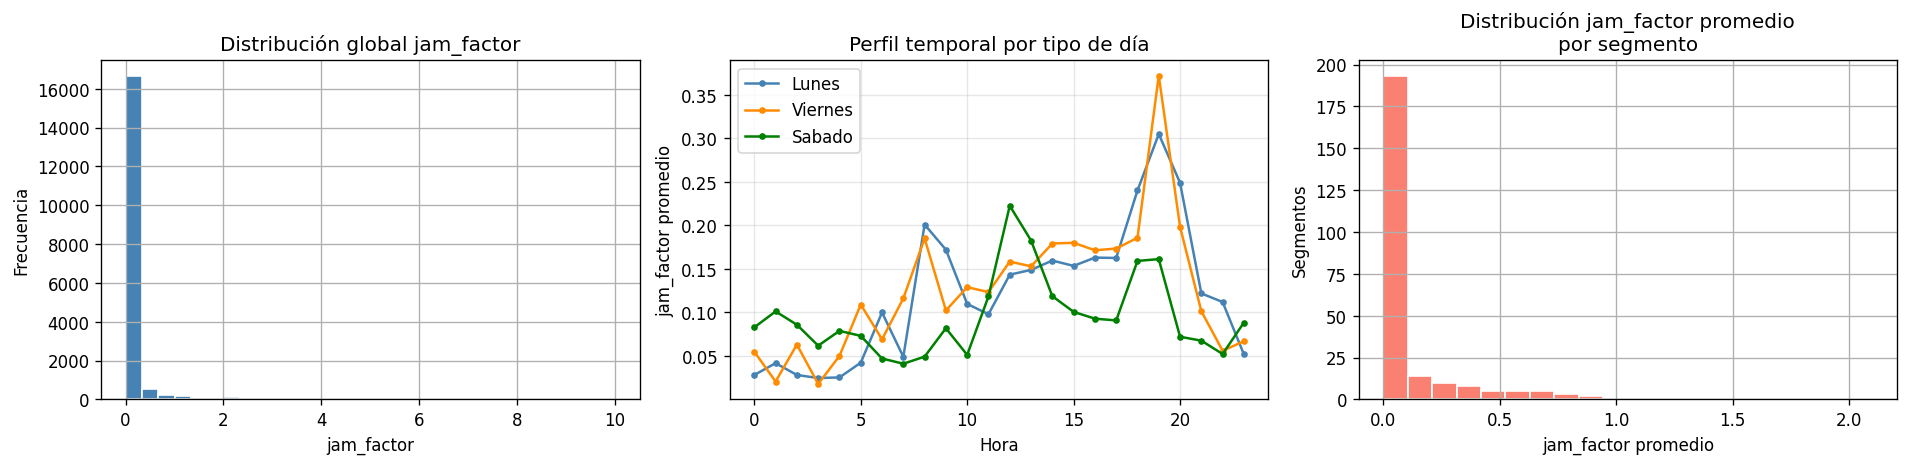
\includegraphics[width=0.90\textwidth]{img/preprocesamiento.png}
  \caption{Distribución global del jam\_factor y perfiles diarios promedio.
           La mayoría de los valores se concentran cerca de 1{,}0 (tráfico fluido),
           con una cola larga hacia valores altos durante las horas pico.}
  \label{fig:preprocesamiento}
\end{figure}

%=================================================================
\section{Modelos no supervisados}
%=================================================================

El aprendizaje no supervisado parte de una premisa sencilla:
\textit{los datos tienen estructura interna} que podemos descubrir sin
necesidad de que alguien nos diga cuál es la respuesta correcta.
En este proyecto usamos seis técnicas complementarias, cada una respondiendo
una pregunta diferente sobre los datos.

%----------------------------------------------------------------
\subsection{PCA --- Reducción de dimensionalidad}
%----------------------------------------------------------------

\subsubsection{Intuición: la sombra más informativa}

Imaginemos que sostenemos un objeto tridimensional (una figura irregular)
frente a una fuente de luz y proyectamos su sombra en una pared.
Según desde qué ángulo pongamos la luz, la sombra mostrará más o menos
detalles del objeto.
\textbf{PCA} (\textit{Principal Component Analysis}) busca
\emph{el ángulo de iluminación que produce la sombra más informativa}:
la proyección que preserva la mayor cantidad de variación entre los puntos.

En nuestro caso, los 250 segmentos son objetos en un espacio de 96
dimensiones (una por hora-día).
Visualizar 96 dimensiones es imposible, y muchas de ellas contienen
información redundante: la congestión del lunes a las 8 h y del miércoles
a las 8 h están altamente correlacionadas.
PCA encuentra las pocas ``direcciones independientes'' que capturan la
mayor parte de esa variación.

\subsubsection{Paso a paso}

\begin{enumerate}[noitemsep]
  \item \textbf{Estandarizar}: cada columna se centra en 0 y se escala a
    varianza 1, para que no dominen las horas con valores más altos.
  \item \textbf{Calcular la covarianza}: se mide cuánto varían juntas cada
    par de columnas. El resultado es la \emph{matriz de covarianza}
    $\Sigma \in \mathbb{R}^{p \times p}$.
  \item \textbf{Descomponer}: se calculan los \emph{eigenvectores}
    de $\Sigma$. Cada eigenvector $v_k$ es una dirección en el espacio
    original, y su eigenvalor $\lambda_k$ indica cuánta varianza captura.
  \item \textbf{Proyectar}: cada segmento se representa como sus coordenadas
    en las $K$ primeras direcciones $\to$ de 96 a 13 números.
\end{enumerate}

\subsubsection{Matemática}

Dado $X \in \mathbb{R}^{n \times p}$ (estandarizado), la varianza explicada
por las primeras $K$ componentes es:

\begin{equation}
  \text{VE}(K) = \frac{\sum_{k=1}^{K} \lambda_k}{\sum_{k=1}^{p} \lambda_k},
  \quad \lambda_1 \geq \lambda_2 \geq \cdots \geq \lambda_p \geq 0
  \label{eq:pca_ve}
\end{equation}

Con $K = 13$ se captura entre el 86\% (La Paz) y el 96\% (El Alto) de
la varianza total. Esto significa que 13 números por segmento describen
casi tan bien su comportamiento como los 96 originales.

\paragraph{¿Qué captura PC1?}
La primera componente principal correlaciona fuertemente con el nivel
general de congestión: segmentos que son congestionados en todas las horas
y días tienen un PC1 alto.
PC2 captura la diferencia entre el patrón de días laborales y el sábado.
Las siguientes componentes capturan patrones cada vez más sutiles
(diferencias entre horas, entre zonas, etc.).

\begin{figure}[H]
  \centering
  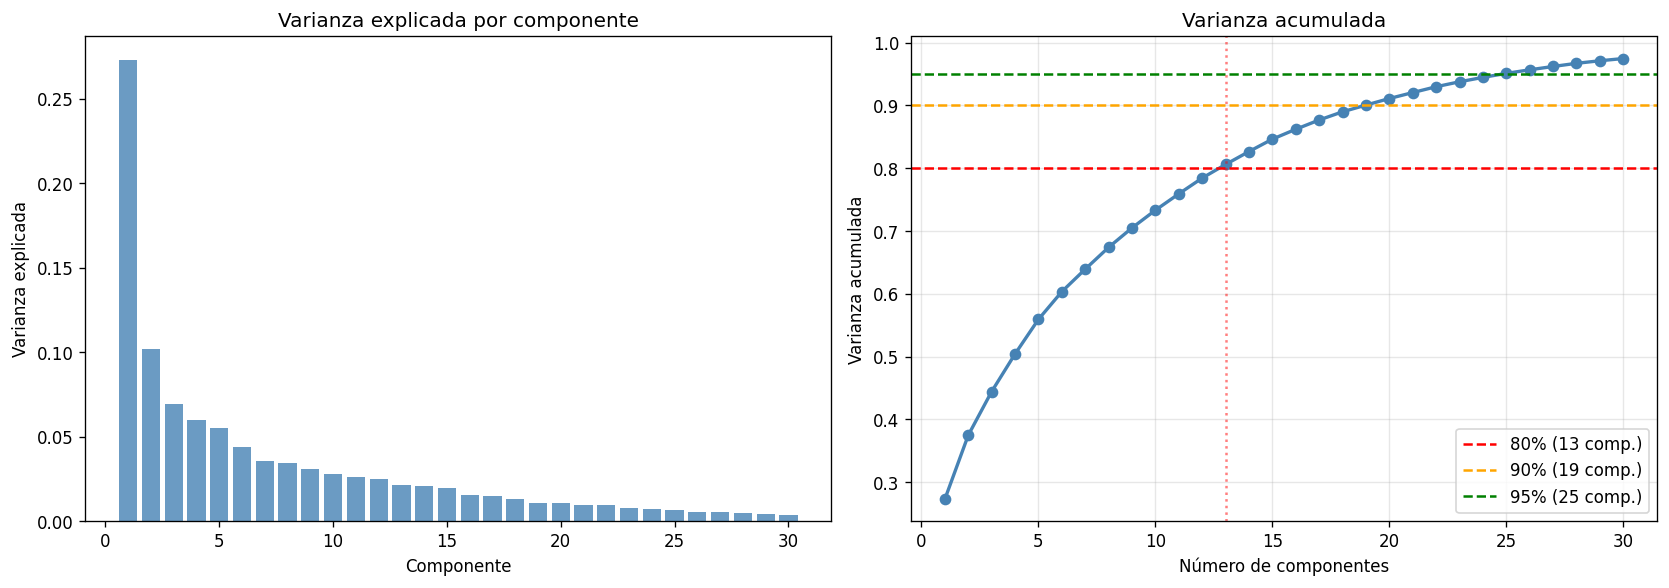
\includegraphics[width=0.88\textwidth]{img/pca_varianza.png}
  \caption{Izquierda: varianza explicada por cada componente principal
           (gráfico de scree). Derecha: varianza acumulada. Con 13
           componentes se supera el umbral del 85\%.}
  \label{fig:pca_varianza}
\end{figure}

\begin{lstlisting}[caption={PCA con sklearn.}]
from sklearn.decomposition import PCA
from sklearn.preprocessing import StandardScaler

X_std = StandardScaler().fit_transform(feat.values)
pca   = PCA(n_components=13, random_state=42)
X_pca = pca.fit_transform(X_std)          # (250, 13)
var_ac = pca.explained_variance_ratio_.cumsum()[-1]
print(f"Varianza acumulada: {var_ac:.1%}")
# La Paz:  86.8%
# El Alto: 96.1%
\end{lstlisting}

%----------------------------------------------------------------
\subsection{UMAP --- Visualización en 2D}
%----------------------------------------------------------------

\subsubsection{Intuición: el mapa del terreno}

PCA es como tomar una fotografía aérea de la nube de puntos: proyecta de
forma \emph{lineal}, sin doblar el espacio.
Pero los datos reales muchas veces viven en una \emph{variedad} (manifold):
una superficie curva embebida en alta dimensión, como la superficie de la
Tierra dentro del espacio 3D.

\textbf{UMAP} (\textit{Uniform Manifold Approximation and Projection})
es como hacer un \emph{mapa cartográfico} de esa superficie curva:
aplana la variedad en 2D intentando que los puntos que eran vecinos en alta
dimensión sigan siendo vecinos en el plano.

La diferencia clave con t-SNE (otro método popular) es que UMAP
\textbf{preserva mejor la estructura global}: no solo agrupa localmente, sino
que mantiene la distancia relativa entre grupos.
Además es considerablemente más rápido.

\subsubsection{El parámetro n\_neighbors: local vs. global}

Imagine que en un barrio nuevo solo conoce a sus 3 vecinos más cercanos.
Su idea del barrio será muy local —solo ve lo que pasa en su manzana.
Si en cambio conoce a sus 50 vecinos más cercanos, tiene una visión más global
—puede detectar patrones de toda la cuadra.

El parámetro \texttt{n\_neighbors} en UMAP funciona igual: un valor pequeño
(ej. 5) hace que UMAP se concentre en estructura muy fina y local; uno grande
(ej. 50) captura la estructura global.
Con \textbf{n\_neighbors = 15} para 250 puntos obtenemos un equilibrio adecuado.

\begin{center}
\begin{tabular}{lll}
  \toprule
  Parámetro & Valor & Efecto \\
  \midrule
  \texttt{n\_neighbors} & 15 & equilibrio local/global para 250 puntos \\
  \texttt{min\_dist} & 0.1 & separación mínima, evita solapamiento \\
  \texttt{n\_components} & 2 & proyección en 2 dimensiones \\
  \bottomrule
\end{tabular}
\end{center}

\begin{figure}[H]
  \centering
  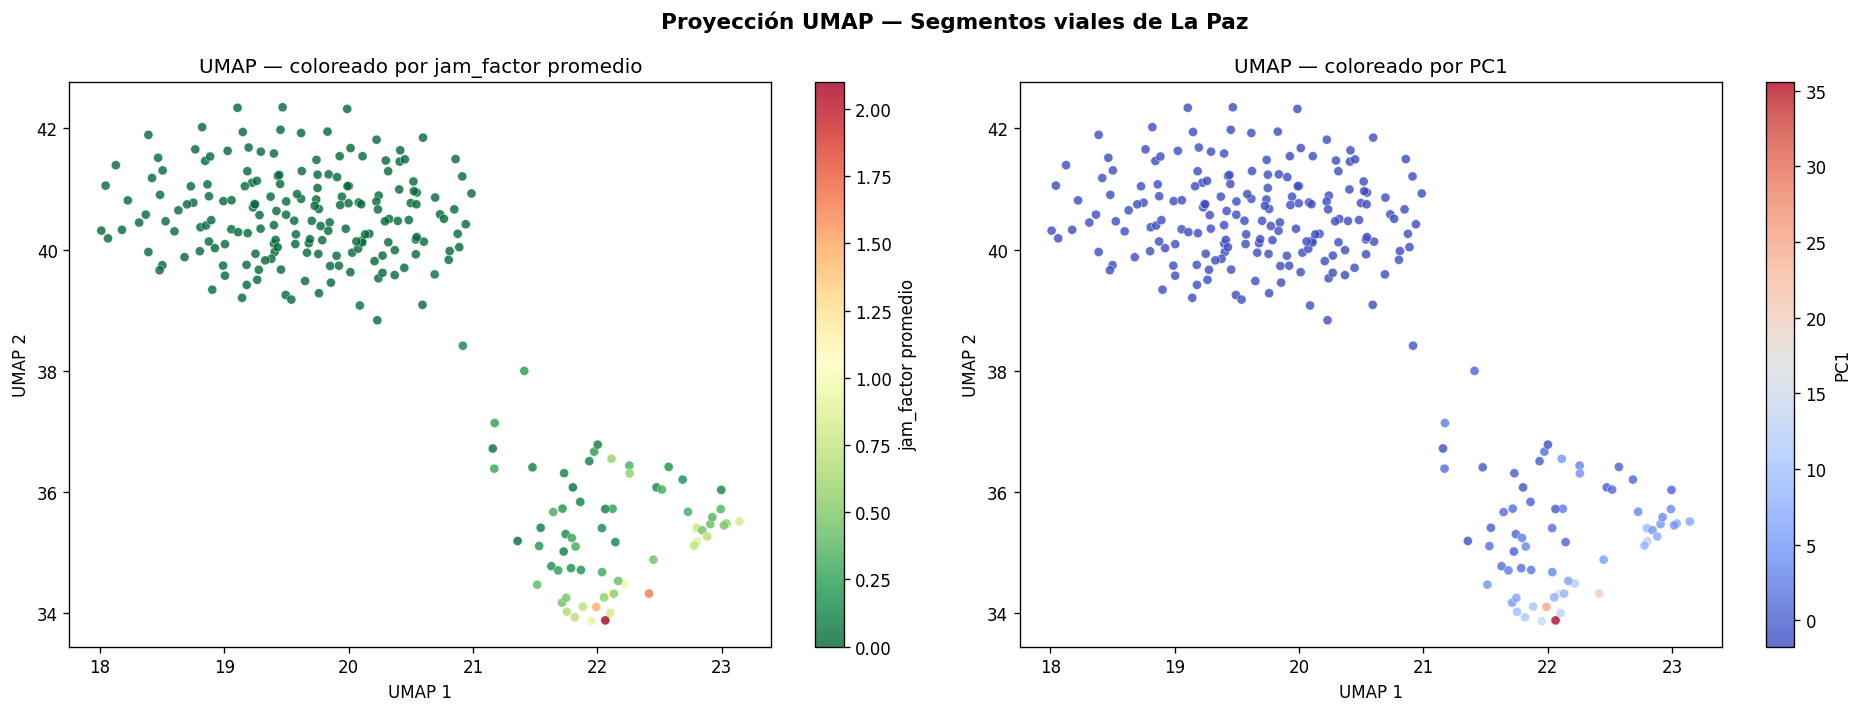
\includegraphics[width=0.88\textwidth]{img/umap_proyeccion.png}
  \caption{Proyección UMAP de los 250 segmentos de La Paz.
           Izquierda: coloreado por jam\_factor medio (rojo = más congestionado).
           Derecha: coloreado por PC1. Los dos grupos visibles corresponden
           a los clusters de alta y baja congestión descubiertos por K-Means.}
  \label{fig:umap}
\end{figure}

\begin{lstlisting}[caption={UMAP sobre las componentes PCA.}]
import umap

reducer = umap.UMAP(n_neighbors=15, min_dist=0.1,
                    n_components=2, random_state=42)
X_umap  = reducer.fit_transform(X_pca)    # (250, 2)
\end{lstlisting}

%----------------------------------------------------------------
\subsection{DBSCAN --- Clustering espacial geográfico}
%----------------------------------------------------------------

\subsubsection{Intuición: islas de densidad}

DBSCAN (\textit{Density-Based Spatial Clustering of Applications with Noise})
parte de una idea geográfica muy natural: un \textbf{barrio} es una zona
donde las casas están relativamente juntas, separada de otros barrios por
áreas más despobladas.

El algoritmo busca ``islas'' de puntos densos separadas por zonas vacías.
Las dos ventajas clave sobre K-Means son:
\begin{enumerate}[noitemsep]
  \item \textbf{No requiere especificar k}: el algoritmo encuentra cuántos
    clusters hay automáticamente.
  \item \textbf{Detecta outliers}: los puntos aislados que no pertenecen
    a ningún grupo se marcan como ruido (valor $-1$).
\end{enumerate}

En este proyecto lo aplicamos sobre las \emph{coordenadas GPS} de los
segmentos para identificar zonas geográficas homogéneas de la ciudad.

\subsubsection{Core points, border points y ruido}

\begin{center}
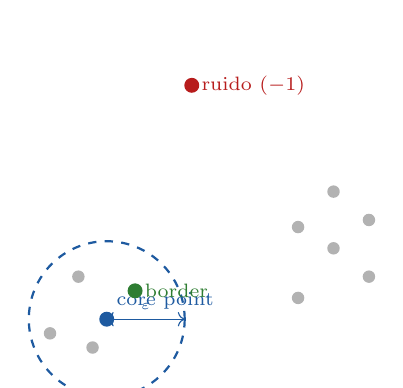
\begin{tikzpicture}[scale=0.9]
  % Puntos de fondo
  \foreach \x/\y in {1/1, 1.4/1.8, 1.8/1.2, 2.2/1.6, 1.6/0.8,
                      4.5/2.5, 5.0/2.2, 5.5/2.6, 5.0/3.0,
                      4.5/1.5, 5.5/1.8,
                      3.0/4.5}{
    \fill[gray!60] (\x,\y) circle (2.5pt);
  }
  % Core point con círculo eps
  \fill[azulAS] (1.8,1.2) circle (3pt);
  \draw[azulAS, dashed, thick] (1.8,1.2) circle (1.1cm);
  \node[azulAS, font=\scriptsize, above right] at (1.8,1.2) {core point};

  % Border point
  \fill[verdePos] (2.2,1.6) circle (3pt);
  \node[verdePos, font=\scriptsize, right] at (2.2,1.6) {border};

  % Outlier / ruido
  \fill[rojoNeg] (3.0,4.5) circle (3pt);
  \node[rojoNeg, font=\scriptsize, right] at (3.0,4.5) {ruido ($-1$)};

  % Etiqueta eps
  \draw[<->, azulAS] (1.8,1.2) -- +(1.1,0)
    node[midway, above, font=\tiny] {$\varepsilon$};
\end{tikzpicture}
\end{center}

Un punto es \textbf{core point} si tiene al menos \texttt{min\_samples}
vecinos en un radio $\varepsilon$.
Los puntos en la frontera de un core point (pero que no lo son ellos mismos)
son \textbf{border points}.
Los puntos que no tienen suficientes vecinos son \textbf{ruido}.

\subsubsection{¿Por qué la distancia haversine?}

La distancia euclidea entre coordenadas GPS ($\Delta\text{lat}, \Delta\text{lon}$)
es imprecisa: 1 grado de longitud en el ecuador mide $\sim$111 km, pero en
latitud $-16°$ (La Paz) mide $\sim$107 km.
La \textbf{fórmula haversine} calcula la distancia real sobre la esfera
terrestre:

\begin{equation}
  d = 2R\arcsin\!\left(\sqrt{
    \sin^2\!\tfrac{\Delta\phi}{2} +
    \cos\phi_1\cos\phi_2\,\sin^2\!\tfrac{\Delta\lambda}{2}
  }\right)
\end{equation}

donde $R = 6\,371\,000$ m, $\phi$ es latitud y $\lambda$ longitud en radianes.

\begin{lstlisting}[caption={DBSCAN haversine con sklearn.}]
from sklearn.cluster import DBSCAN
import numpy as np

EARTH_RADIUS_M = 6_371_000
coords_rad = np.radians(segs[["lat", "lon"]].values)

db = DBSCAN(
    eps=500 / EARTH_RADIUS_M,   # 500 m en radianes
    min_samples=5,
    metric="haversine"
)
cluster_espacial = db.fit_predict(coords_rad)
\end{lstlisting}

\subsubsection{Resultados del clustering espacial}

Aplicando DBSCAN sobre los centroides GPS de los 250 segmentos de La Paz,
el algoritmo identificó \textbf{11 clusters} y clasificó el 68\,\% de los
segmentos (170/250) como ruido ($-1$).
El índice de silueta sobre los puntos asignados (no-ruido) fue de
\textbf{0{,}681}, indicando buena cohesión interna dentro de las zonas
encontradas.

\begin{center}
\begin{tabular}{lc}
  \toprule
  Resultado & Valor \\
  \midrule
  Clusters encontrados     & 11 \\
  Segmentos asignados      & 80 (32\,\%) \\
  Segmentos como ruido     & 170 (68\,\%) \\
  Silueta (no-ruido)       & 0{,}681 \\
  \bottomrule
\end{tabular}
\end{center}

El alto porcentaje de ruido no es un fallo del modelo, sino una consecuencia
directa de la densidad de monitoreo.
Con 250 segmentos distribuidos sobre $\sim$2\,167\,km de red vial,
cada punto monitoreado tiene en promedio \textbf{2{,}1 vecinos} dentro de
un radio de 500\,m, muy por debajo del umbral \texttt{min\_samples=5}.
Solo en las zonas donde el muestreo estratificado concentró varios segmentos
cercanos se forman clusters; esas son precisamente las 11 zonas identificadas.

\medskip
\noindent\textbf{Nota de interpretación.}
Los clusters DBSCAN no detectan zonas de congestión sino zonas de
\emph{cobertura densa} del monitoreo.
Su valor analítico está en cruzarse con K-Means: un cluster DBSCAN donde
todos los segmentos son de alta congestión temporal indica una zona
geográfica homogéneamente congestionada; uno mixto sugiere heterogeneidad
intra-zona.
Esta combinación de geografía (DBSCAN) y comportamiento temporal (K-Means)
ofrece una caracterización más completa que cualquiera de los dos solos.

%----------------------------------------------------------------
\subsection{K-Means --- Clustering temporal}
%----------------------------------------------------------------

\subsubsection{Intuición: el proceso de asignación iterativa}

Imagine que tiene que dividir 250 alumnos en 2 grupos equilibrados según
su rendimiento en 96 exámenes.
Una estrategia es:
\begin{enumerate}[noitemsep]
  \item Elegir 2 alumnos al azar como ``representantes'' iniciales.
  \item Asignar cada alumno al representante más parecido.
  \item Reemplazar cada representante por el promedio de su grupo.
  \item Repetir desde el paso 2 hasta que los grupos no cambien.
\end{enumerate}

K-Means hace exactamente esto, pero con vectores de 96 dimensiones
(perfil completo de tráfico por hora-día) y como medida de similitud
usa la distancia euclídea.

\subsubsection{La función de costo}

K-Means minimiza la suma total de distancias al cuadrado entre cada punto
y el centroide de su cluster:

\begin{equation}
  J = \sum_{j=1}^{k} \sum_{i \in C_j}
  \left\| x_i - \mu_j \right\|^2
  \label{eq:kmeans}
\end{equation}

donde $\mu_j$ es el centroide del cluster $j$ y $C_j$ el conjunto de
puntos asignados a ese cluster.

\subsubsection{Elección de k: el método del codo}

Para elegir $k$ graficamos la función de costo $J$ en función del número
de clusters.
Al agregar más clusters, $J$ siempre baja (más grupos $\to$ segmentos
más cerca de su centroide).
Pero hay un punto donde la mejora se vuelve marginal: el ``codo'' de la
curva.
Complementamos con el \textbf{índice de silueta}, que mide qué tan bien
separados están los clusters ($1 = $ perfectamente separados, $0 = $ solapados).

\begin{figure}[H]
  \centering
  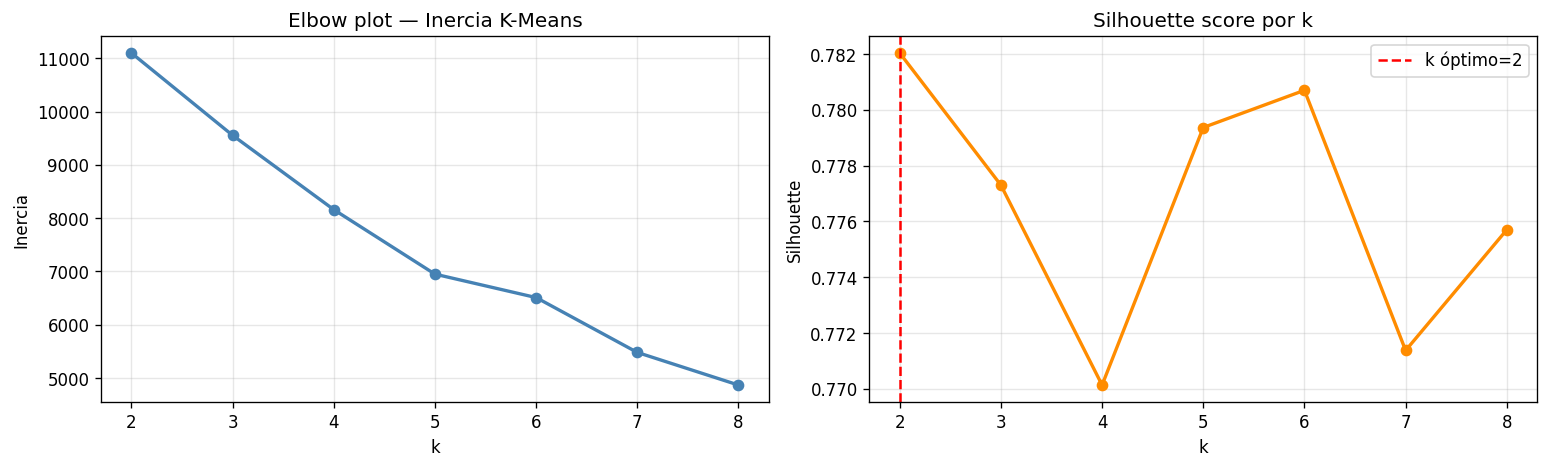
\includegraphics[width=0.82\textwidth]{img/kmeans_codo.png}
  \caption{Método del codo (inercia vs.~$k$) e índice de silueta.
           Ambos indicadores señalan $k=2$ como el número óptimo de clusters:
           el codo se forma en $k=2$ y la silueta alcanza su máximo.}
  \label{fig:kmeans_codo}
\end{figure}

\begin{lstlisting}[caption={K-Means temporal con validación.}]
from sklearn.cluster import KMeans
from sklearn.metrics import silhouette_score

# Elegir k evaluando inercia y silueta
for k in range(2, 8):
    km  = KMeans(n_clusters=k, random_state=42, n_init=20)
    lbl = km.fit_predict(X_std)
    sil = silhouette_score(X_std, lbl)
    print(f"k={k}: inercia={km.inertia_:.1f}, silueta={sil:.3f}")

# k=2 elegido: inercia cae bruscamente, silueta maxima
km = KMeans(n_clusters=2, random_state=42, n_init=20)
cluster_temporal = km.fit_predict(X_std)
\end{lstlisting}

El parámetro \texttt{n\_init=20} reinicia el algoritmo 20 veces con
centroides iniciales distintos y se queda con la mejor solución, evitando
mínimos locales.

\begin{figure}[H]
  \centering
  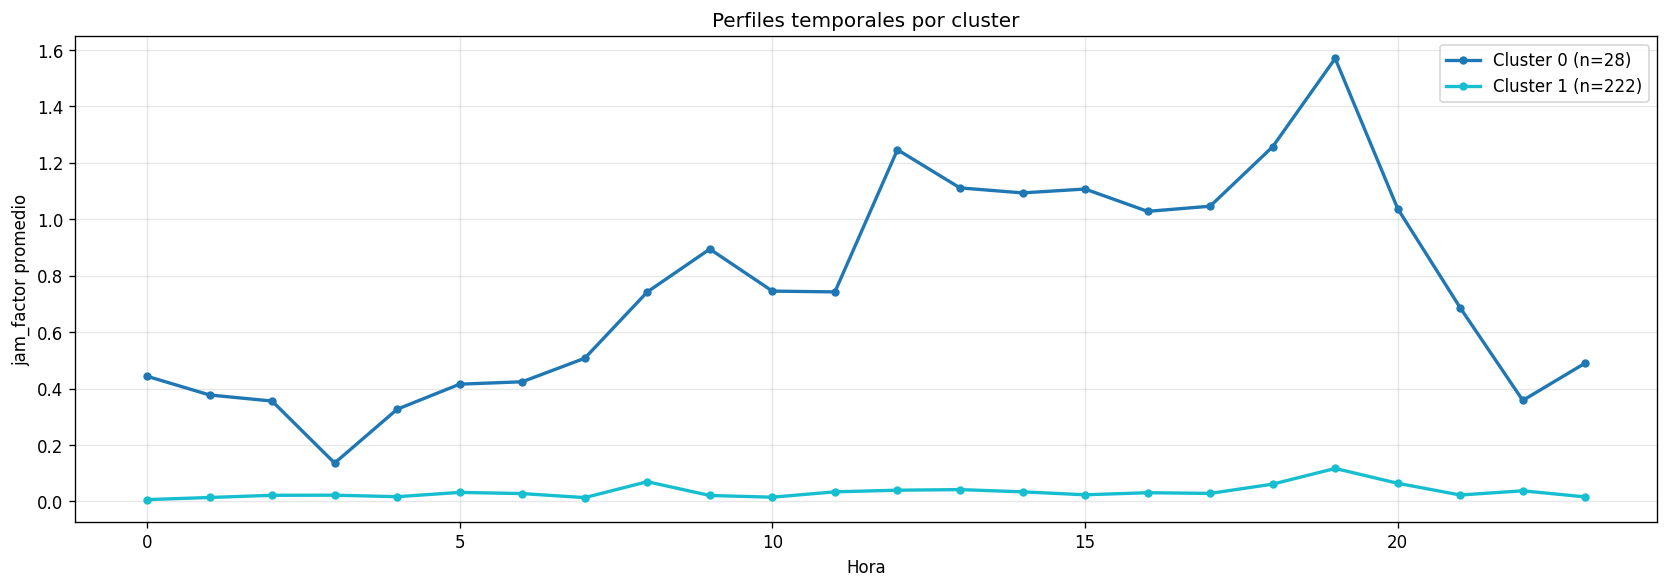
\includegraphics[width=0.88\textwidth]{img/perfiles_clusters.png}
  \caption{Perfil promedio de jam\_factor por hora para cada cluster temporal.
           El cluster 0 (alta congestión) muestra picos pronunciados en hora
           pico; el cluster 1 (baja congestión) mantiene valores próximos
           a 1{,}0 durante todo el día.}
  \label{fig:perfiles_clusters}
\end{figure}

\subsubsection{Resultados del clustering}

El índice de silueta obtenido con $k=2$ fue de \textbf{0{,}766}, indicando
clusters bien separados y compactos en el espacio PCA de 13 dimensiones.
Este valor valida cuantitativamente la elección de $k=2$: los dos grupos
no son una conveniencia del algoritmo sino estructuras genuinas en los datos.

\begin{center}
\begin{tabular}{lrrrrc}
  \toprule
  Zona & \multicolumn{2}{c}{Alta congestión} & \multicolumn{2}{c}{Baja congestión} & Silueta \\
       & $n$ & \% & $n$ & \% & \\
  \midrule
  La Paz  & 27  & 10{,}8 & 223 & 89{,}2 & 0{,}766 \\
  El Alto & 10  &  4{,}0 & 240 & 96{,}0 & --- \\
  \bottomrule
\end{tabular}
\end{center}

La Paz tiene casi el triple de proporción de segmentos de alta congestión
que El Alto (10{,}8\,\% vs.\ 4{,}0\,\%).
Esta diferencia refleja condiciones estructurales: La Paz está construida
en una hoya cordillerana con calles estrechas, alta densidad de
intersecciones y un centro histórico donde convergen las principales
arterias.
El Alto, en cambio, fue planificado en cuadrícula sobre el altiplano con
avenidas más anchas y menos cuellos de botella topográficos.

\medskip
\textbf{Perfil temporal del cluster de alta congestión.}
El análisis de los perfiles horarios revela un patrón bimodal consistente:
pico matutino a las \textbf{08:00} (jam $\approx 0{,}201$ en lunes) y pico
vespertino a las \textbf{19:00} (jam máximo = 0{,}372 el viernes).
Los sábados el pico matutino cae a jam $\approx 0{,}049$, confirmando que
la congestión severa es un fenómeno de día hábil.
El cluster de baja congestión no supera jam $\approx 0{,}3$ en ningún horario
ni día, lo que justifica la separación binaria.

La congestión severa está concentrada en un subconjunto pequeño de
arterias: el centro histórico, la Av.\ Montes y la autopista La Paz--El
Alto; la Ceja y la Av.\ 6 de Marzo en El Alto.

\begin{figure}[H]
  \centering
  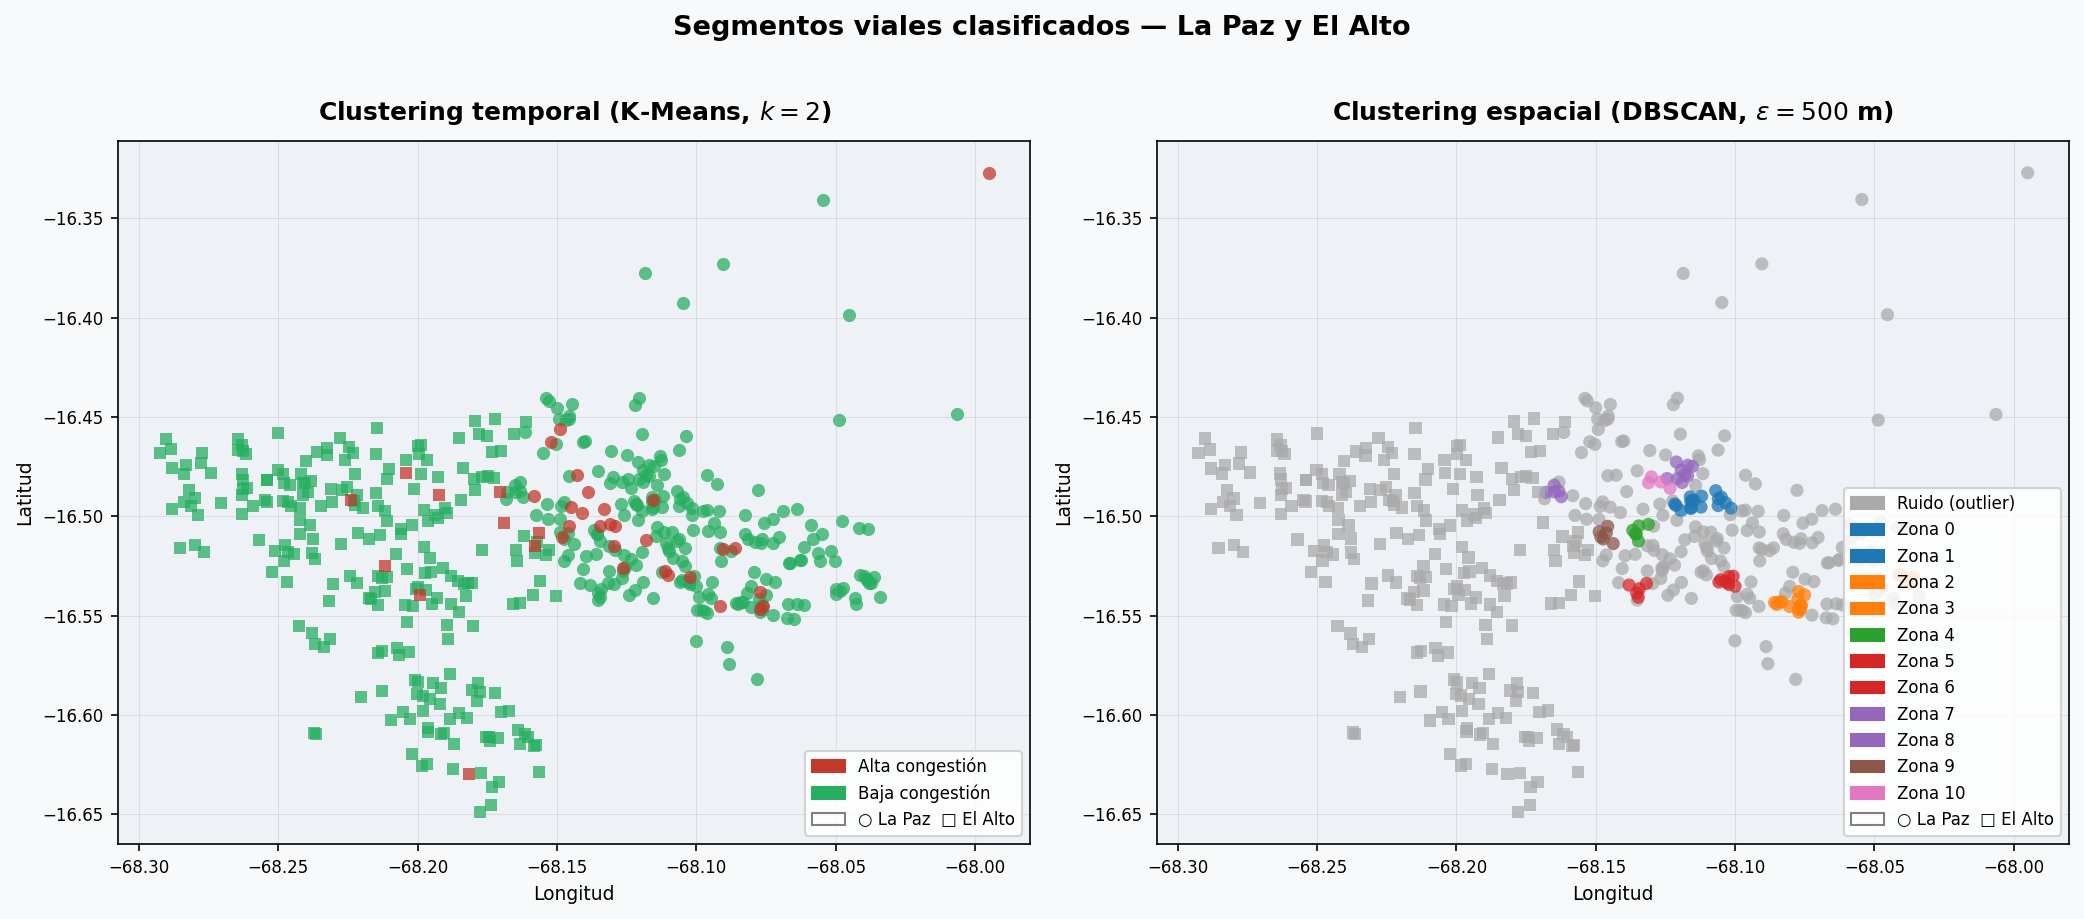
\includegraphics[width=0.92\textwidth]{img/mapa_clusters.png}
  \caption{Distribución geográfica de los clusters.
           \textbf{Izquierda}: clustering temporal K-Means (rojo=alta congestión,
           verde=baja congestión). \textbf{Derecha}: clustering espacial DBSCAN
           (zonas geográficas). Los cuadrados corresponden a El Alto
           (altiplano, latitudes más altas) y los círculos a La Paz (hoya).}
  \label{fig:mapa_clusters}
\end{figure}

%----------------------------------------------------------------
\subsection{NMF --- Síntesis de días faltantes}
%----------------------------------------------------------------

\subsubsection{El problema}

Solo se recolectaron 4 días (lunes, miércoles, viernes, sábado).
Martes, jueves y domingo quedaron sin datos.
Para completar la semana sin consumir cuota de API, usamos un modelo no
supervisado de \textbf{factorización matricial}.

\subsubsection{Intuición: los arquetipos del tráfico}

Imagine que la congestión de una ciudad puede explicarse con 6
``arquetipos'' (patrones puros):

\begin{enumerate}[noitemsep]
  \item El \textbf{ritmo del centro}: alto mediodía, alto hora pico.
  \item El \textbf{ritmo de la autopista}: solo en las entradas/salidas del día.
  \item El \textbf{ritmo residencial}: casi siempre tranquilo, leve pico matutino.
  \item El \textbf{ritmo comercial}: activo desde las 9 h hasta las 20 h.
  \item El \textbf{ritmo universitario}: activo en horarios de clases.
  \item El \textbf{ritmo nocturno}: activo en zonas de vida nocturna.
\end{enumerate}

Cada segmento real es una \emph{mezcla} de estos arquetipos.
NMF encuentra los arquetipos ($H$) y las proporciones de cada segmento ($W$).

\subsubsection{Matemática de NMF}

NMF (\textit{Non-negative Matrix Factorization}) descompone la matriz $X$ como:

\begin{equation}
  X \approx W \cdot H,
  \quad W \geq 0,\; H \geq 0
  \label{eq:nmf}
\end{equation}

\begin{center}
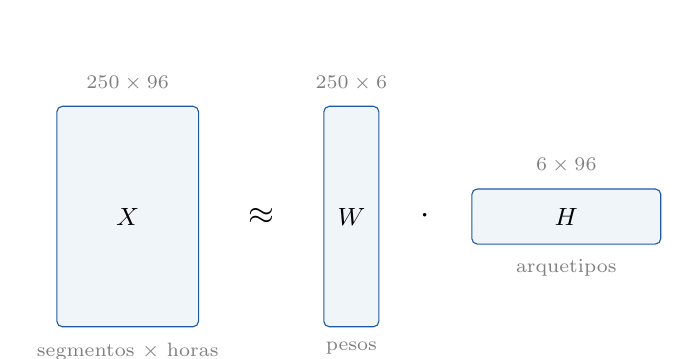
\begin{tikzpicture}[
  mat/.style={rectangle, draw=azulAS, fill=grisCelda, rounded corners=2pt,
              minimum width=1.2cm, minimum height=2.8cm, font=\small},
  arr/.style={->, >=Stealth, thick, color=azulAS},
  lbl/.style={font=\scriptsize, color=gray}
]
  \node[mat, minimum width=1.8cm] (X) {$X$};
  \node[lbl, above=2pt of X] {$250\times 96$};
  \node[lbl, below=2pt of X] {segmentos $\times$ horas};

  \node[font=\large, right=0.5cm of X] (eq) {$\approx$};

  \node[mat, minimum width=0.7cm, right=0.5cm of eq] (W) {$W$};
  \node[lbl, above=2pt of W] {$250\times 6$};
  \node[lbl, below=2pt of W] {pesos};

  \node[font=\large, right=0.4cm of W] (dot) {$\cdot$};

  \node[mat, minimum width=2.4cm, minimum height=0.7cm,
        right=0.4cm of dot] (H) {$H$};
  \node[lbl, above=2pt of H] {$6\times 96$};
  \node[lbl, below=2pt of H] {arquetipos};
\end{tikzpicture}
\end{center}

La restricción de \textbf{no negatividad} ($W,H \geq 0$) es fundamental:
el jam\_factor siempre es positivo, por lo que tiene sentido que los
arquetipos y los pesos sean positivos.
PCA, en cambio, genera componentes con valores negativos que no tienen
interpretación directa en este contexto.

\begin{center}
\begin{tabular}{lcc}
  \toprule
  Característica & NMF & PCA \\
  \midrule
  Valores en componentes & solo positivos & positivos y negativos \\
  Interpretabilidad & alta (partes aditivas) & media \\
  No-negatividad garantizada & sí & no \\
  Unicidad de la solución & no siempre & sí \\
  \bottomrule
\end{tabular}
\end{center}

\subsubsection{Pipeline NMF + PCHIP}

\begin{center}
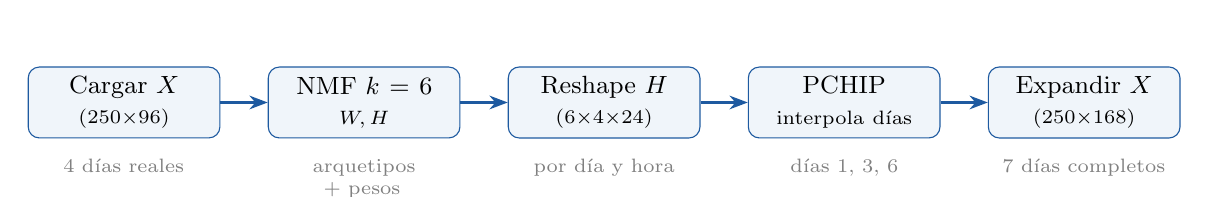
\begin{tikzpicture}[
  node distance=0.6cm and 0.6cm,
  pstep/.style={rectangle, rounded corners=4pt, draw=azulAS, fill=grisCelda,
               text width=2.2cm, minimum height=0.9cm, text centered, font=\small},
  sub/.style={font=\scriptsize, color=gray, text width=2.2cm, text centered},
  arr/.style={->, >=Stealth, thick, color=azulAS}
]
  \node[pstep] (load) {Cargar $X$\\\scriptsize(250$\times$96)};
  \node[pstep, right=of load] (nmf) {NMF $k=6$\\\scriptsize $W, H$};
  \node[pstep, right=of nmf] (reshape) {Reshape $H$\\\scriptsize(6$\times$4$\times$24)};
  \node[pstep, right=of reshape] (pchip) {PCHIP\\\scriptsize interpola días};
  \node[pstep, right=of pchip] (expand) {Expandir $X$\\\scriptsize(250$\times$168)};

  \draw[arr] (load) -- (nmf);
  \draw[arr] (nmf) -- (reshape);
  \draw[arr] (reshape) -- (pchip);
  \draw[arr] (pchip) -- (expand);

  \node[sub, below=4pt of load] {4 días reales};
  \node[sub, below=4pt of nmf] {arquetipos + pesos};
  \node[sub, below=4pt of reshape] {por día y hora};
  \node[sub, below=4pt of pchip] {días 1, 3, 6};
  \node[sub, below=4pt of expand] {7 días completos};
\end{tikzpicture}
\end{center}

\subsubsection{Los 6 arquetipos encontrados}

Una vez entrenado el modelo, cada fila de $H$ es el perfil horario
(24 h) de un arquetipo puro.
Los 6 arquetipos identificados sobre los datos reales se interpretan así:

\begin{center}
\begin{tabular}{clll}
  \toprule
  Arq. & Hora pico & Descripción interpretada & Tipo de segmento dominante \\
  \midrule
  A0 & 19:00 & Salida laboral vespertina    & Arterias principales \\
  A1 & 08:00 & Entrada laboral matutina     & Accesos al centro \\
  A2 & 17:00 & Tarde laboral                & Comercial/mixto \\
  A3 & 14:00 & Actividad comercial mediodía & Zonas de mercado \\
  A4 & 07:00 & Madrugada (servicios)        & Logística / distribución \\
  A5 & 12:00 & Pausa del mediodía           & Barrios residenciales \\
  \bottomrule
\end{tabular}
\end{center}

Cada segmento es combinación lineal de estos arquetipos, codificada en
su fila de $W$.
Un segmento con $W_{i,1}$ dominante es, por construcción, un segmento de
\emph{entrada matutina}: independientemente del día que se observe, su
perfil siempre tendrá el pico alrededor de las 08:00.
La no-negatividad garantiza que estas proporciones sean directamente
interpretables como contribuciones aditivas al jam\_factor.

\medskip
\textbf{Conexión con K-Means.}
Los arquetipos NMF son los bloques constructivos del tráfico.
K-Means agrupa segmentos según cuáles arquetipos dominan su comportamiento
semanal completo: los segmentos de alta congestión tienden a concentrar
peso en A0 y A1 (picos laborales intensos), mientras que los de baja
congestión muestran pesos distribuidos en A3--A5 (patrones más suaves).
La coherencia entre ambas caracterizaciones valida la robustez del análisis.

%----------------------------------------------------------------
\subsection{PCHIP --- Interpolación día-de-semana}
%----------------------------------------------------------------

\subsubsection{Intuición: la curva que no oscila}

Una vez que NMF nos da los arquetipos para los 4 días conocidos
(posiciones 0, 2, 4, 5 en la semana), necesitamos \emph{estimar} los
arquetipos para martes (posición 1), jueves (3) y domingo (6).

El problema es conectar puntos con una curva suave.
Existen varias opciones:

\begin{itemize}[noitemsep]
  \item \textbf{Interpolación lineal}: une los puntos con líneas rectas.
    Simple, pero poco realista (cambios bruscos).
  \item \textbf{Spline cúbico}: curva muy suave, pero puede oscilar
    (\textit{ringing}) entre puntos, especialmente al extrapolar fuera
    del rango conocido.
  \item \textbf{PCHIP} (\textit{Piecewise Cubic Hermite Interpolating
    Polynomial}): curva cúbica monotone-preserving. Entre dos puntos
    consecutivos no crea picos o valles artificiales.
\end{itemize}

\begin{center}
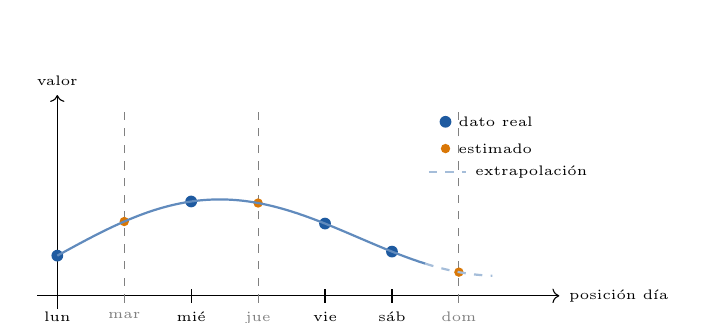
\begin{tikzpicture}[scale=0.85]
  % Eje x
  \draw[->] (-0.3,0) -- (7.5,0) node[right, font=\tiny] {posición día};
  \draw[->] (0,-0.2) -- (0,3.0) node[above, font=\tiny] {valor};

  % Etiquetas días
  \foreach \x/\lbl in {0/lun, 2/mié, 4/vie, 5/sáb} {
    \draw (\x, -0.1) -- (\x, 0.1);
    \node[font=\tiny, below] at (\x, -0.1) {\lbl};
    \fill[azulAS] (\x, {0.6+0.7*sin(\x*40)+0.3*\x*0.2}) circle (2.5pt);
  }
  % Días sintéticos
  \foreach \x/\lbl in {1/mar, 3/jue, 6/dom} {
    \draw[dashed, gray] (\x, -0.1) -- (\x, 2.8);
    \node[font=\tiny, below, gray] at (\x, -0.1) {\lbl};
    \fill[naranjaAdv] (\x, {0.6+0.7*sin(\x*40)+0.3*\x*0.2}) circle (2pt);
  }
  % Curva PCHIP aproximada
  \draw[azulAS!70, thick, smooth]
    plot[domain=0:5.5, samples=60] (\x, {0.6+0.7*sin(\x*40)+0.3*\x*0.2});
  \draw[azulAS!40, dashed, thick, smooth]
    plot[domain=5.5:6.5, samples=20] (\x, {0.6+0.7*sin(\x*40)+0.3*\x*0.2});

  % Leyenda
  \fill[azulAS] (5.8,2.6) circle (2.5pt);
  \node[font=\tiny, right] at (5.85,2.6) {dato real};
  \fill[naranjaAdv] (5.8,2.2) circle (2pt);
  \node[font=\tiny, right] at (5.85,2.2) {estimado};
  \draw[azulAS!40, dashed] (5.55,1.85) -- (6.1,1.85);
  \node[font=\tiny, right] at (6.1,1.85) {extrapolación};
\end{tikzpicture}
\end{center}

El \textbf{domingo} (posición 6) queda \emph{fuera} del rango de datos
reales (0--5), lo que lo convierte en una \textbf{extrapolación}.
La extrapolación es inherentemente más incierta que la interpolación
(adivinar fuera de los datos conocidos vs. entre ellos),
razón por la que el domingo se etiqueta con \textbf{confianza baja}.

\begin{lstlisting}[caption={Interpolación PCHIP en el eje día-de-semana.}]
from scipy.interpolate import PchipInterpolator

# Posiciones de los dias reales en la semana (0=lunes, 6=domingo)
pos_reales = [0, 2, 4, 5]   # lunes, mie, vie, sab
pos_sint   = [1, 3, 6]      # martes, jueves, domingo

H_sint = np.zeros((NMF_K, 3, 24))
for ki in range(NMF_K):
    for h in range(24):
        sp = PchipInterpolator(pos_reales, H[ki, :, h])
        H_sint[ki, :, h] = sp(pos_sint)

H_sint = np.clip(H_sint, 0, None)   # garantizar no-negatividad
\end{lstlisting}

\subsubsection{Validación cruzada interna}

Antes de sintetizar los días faltantes, evaluamos la calidad del método
\textbf{ocultando el miércoles} y reconstruyéndolo a partir de
\{lunes (0), viernes (4), sábado (5)\}:

\begin{equation}
  \text{RMSE}_{\text{CV}} =
  \sqrt{\frac{1}{250 \times 24}
    \sum_{i,h} \left(X_{i,\text{mié},h} - \hat{X}_{i,\text{mié},h}\right)^2}
\end{equation}

\begin{center}
\begin{tabular}{lcc}
  \toprule
  Zona & RMSE$_{\text{CV}}$ & Nivel de confianza \\
  \midrule
  La Paz  & 0.462 & conservador (salto de 4 posiciones) \\
  El Alto & 0.435 & conservador (salto de 4 posiciones) \\
  \bottomrule
\end{tabular}
\end{center}

\begin{advbox}
  \textbf{¿Por qué el RMSE es relativamente alto?}
  El CV oculta miércoles (posición 2) y lo predice desde lunes (0),
  viernes (4) y sábado (5) — un \emph{salto de 4 posiciones}.
  Martes y jueves tienen días vecinos a distancia 1,
  por lo que su RMSE real es considerablemente menor.
  El valor reportado es una \textbf{cota superior} conservadora de la calidad.
\end{advbox}

\subsubsection{Nivel de confianza por día}

\begin{center}
\begin{tabular}{lllc}
  \toprule
  Día & Tipo & Posición & Confianza \\
  \midrule
  Lunes     & Real         & 0 & Alta \\
  Martes    & Interpolado  & 1 & Media \\
  Miércoles & Real         & 2 & Alta \\
  Jueves    & Interpolado  & 3 & Media \\
  Viernes   & Real         & 4 & Alta \\
  Sábado    & Real         & 5 & Alta \\
  Domingo   & Extrapolado  & 6 & Baja \\
  \bottomrule
\end{tabular}
\end{center}

%=================================================================
\section{Pipeline completo y decisiones de diseño}
%=================================================================

\subsection{Flujo de datos}

\begin{center}
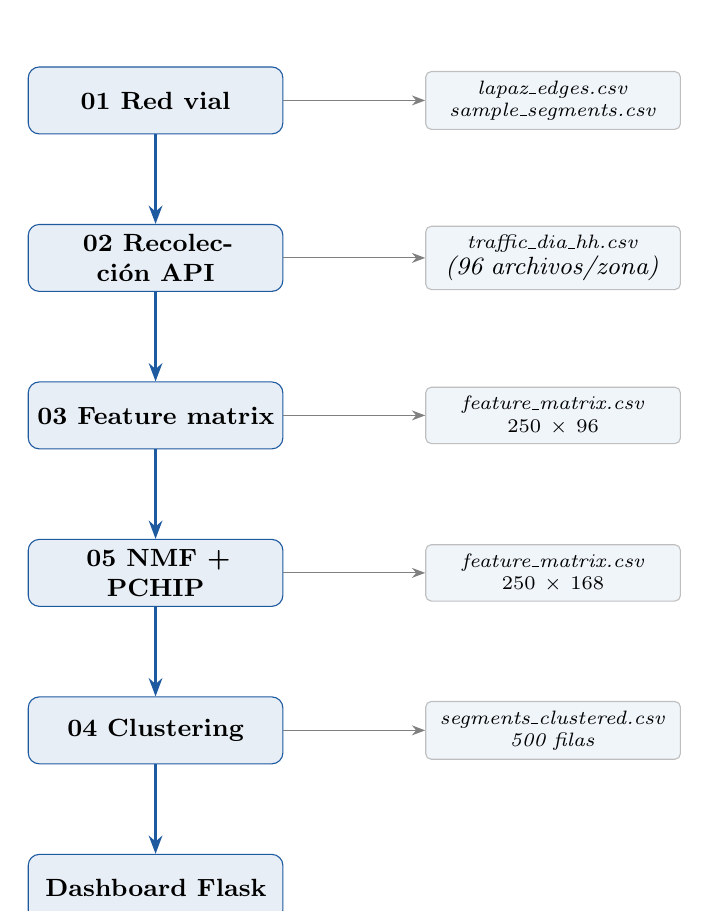
\begin{tikzpicture}[
  node distance=0.0cm and 0.0cm,
  script/.style={rectangle, rounded corners=4pt, draw=azulAS, fill=azulAS!10,
                 text width=3.0cm, minimum height=0.85cm, text centered,
                 font=\small\bfseries},
  iofile/.style={rectangle, rounded corners=2pt, draw=gray!50, fill=grisCelda,
                 text width=3.0cm, minimum height=0.65cm, text centered,
                 font=\scriptsize\itshape},
  arr/.style={->, >=Stealth, thick, color=azulAS},
  ioarr/.style={->, >=Stealth, thin, color=gray}
]
  % Scripts (columna central)
  \node[script] (s01) at (0,0) {01 Red vial};
  \node[script] (s02) at (0,-2.0) {02 Recolección API};
  \node[script] (s03) at (0,-4.0) {03 Feature matrix};
  \node[script] (s05) at (0,-6.0) {05 NMF + PCHIP};
  \node[script] (s04) at (0,-8.0) {04 Clustering};
  \node[script] (dash) at (0,-10.0) {Dashboard Flask};

  \draw[arr] (s01) -- (s02);
  \draw[arr] (s02) -- (s03);
  \draw[arr] (s03) -- (s05);
  \draw[arr] (s05) -- (s04);
  \draw[arr] (s04) -- (dash);

  % Archivos salida (columna derecha)
  \node[iofile, right=1.8cm of s01] (f01) {lapaz\_edges.csv\\sample\_segments.csv};
  \node[iofile, right=1.8cm of s02] (f02) {traffic\_dia\_hh.csv\\\small(96 archivos/zona)};
  \node[iofile, right=1.8cm of s03] (f03) {feature\_matrix.csv\\$250\times 96$};
  \node[iofile, right=1.8cm of s05] (f05) {feature\_matrix.csv\\$250\times 168$};
  \node[iofile, right=1.8cm of s04] (f04) {segments\_clustered.csv\\500 filas};

  \draw[ioarr] (s01.east) -- (f01.west);
  \draw[ioarr] (s02.east) -- (f02.west);
  \draw[ioarr] (s03.east) -- (f03.west);
  \draw[ioarr] (s05.east) -- (f05.west);
  \draw[ioarr] (s04.east) -- (f04.west);
\end{tikzpicture}
\end{center}

\subsection{Decisiones de diseño no obvias}

\begin{description}
  \item[\textbf{250 segmentos por zona, no más.}]
    La API tiene un costo de $\sim$\$5 por 1\,000 consultas.
    Con 250 segmentos $\times$ 24 h $\times$ 4 días $= 24\,000$ consultas por zona
    ($\approx$\$120 total), el costo es manejable y la muestra es representativa.

  \item[\textbf{NMF sobre PCA para síntesis de días.}]
    jam\_factor $\geq 1$: nunca puede ser negativo.
    PCA genera componentes con valores negativos que, al reconstruir,
    podría producir jam\_factors $< 0$ (sin sentido físico).
    NMF garantiza que $W, H \geq 0$, por lo que $WH \geq 0$ siempre.

  \item[\textbf{PCHIP sobre spline cúbico.}]
    El domingo (posición 6) es extrapolación fuera del rango [0--5].
    El spline cúbico estándar puede generar oscilaciones grandes al
    extrapolar. PCHIP es monotone-preserving: no crea picos artificiales,
    produciendo una estimación más conservadora y creíble.

  \item[\textbf{k=6 arquetipos en NMF.}]
    Elegido por balance entre interpretabilidad (pocos arquetipos) y
    fidelidad de reconstrucción (el RMSE de reconstrucción cae rápidamente
    hasta k=6 y luego muy lentamente). Con k=6 el RMSE de reconstrucción
    baja de 0.03 (vs. jam\_mean $\approx 0.18$).

  \item[\textbf{DBSCAN con eps=500 m.}]
    500 m es la distancia a pie en $\sim$6 minutos: calles que están
    en el mismo ``barrio'' a escala peatonal.
    A esta escala, los segmentos del centro histórico forman un cluster
    coherente separado de los barrios periféricos.
\end{description}

%=================================================================
\section{Dashboard interactivo}
%=================================================================

\subsection{Arquitectura}

El dashboard está construido con \textbf{Flask} (servidor web Python) y
\textbf{Folium} (mapas Leaflet.js interactivos en el navegador).

\begin{center}
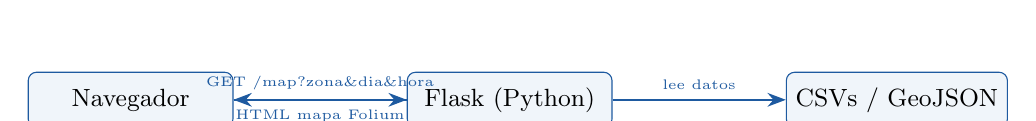
\begin{tikzpicture}[
  box/.style={rectangle, draw=azulAS, fill=grisCelda, rounded corners=3pt,
              text centered, font=\small, minimum width=2.6cm, minimum height=0.7cm},
  arr/.style={->, >=Stealth, thick, color=azulAS}
]
  \node[box] (user) {Navegador};
  \node[box, right=2.2cm of user] (flask) {Flask (Python)};
  \node[box, right=2.2cm of flask] (data) {CSVs / GeoJSON};

  \draw[arr] (user.east) -- node[above, font=\tiny]{GET /map?zona\&dia\&hora}
             (flask.west);
  \draw[arr] (flask.east) -- node[above, font=\tiny]{lee datos}
             (data.west);
  \draw[arr] (flask.west) -- node[below, font=\tiny]{HTML mapa Folium}
             (user.east);
\end{tikzpicture}
\end{center}

Cuando el usuario mueve el slider de hora, el JS del navegador hace un
\texttt{fetch()} a \texttt{/map}, Flask construye un mapa Folium en memoria
y devuelve el HTML como respuesta.
El mapa se embebe en un \texttt{<iframe>} y la comunicación entre iframe y
página usa \texttt{postMessage}.

\subsection{Extensión de calles por nombre}

Un problema visual: solo 250 de $\sim$37\,100 segmentos están en la muestra,
lo que hace que las avenidas aparezcan como puntos aislados en el mapa.
Solución: se carga un GeoJSON con \emph{todos} los segmentos de la red,
y a cada uno que comparte nombre con un segmento muestreado se le asigna
el color de ese segmento (con opacidad reducida).
Esto extiende visualmente las avenidas sin duplicar datos de tráfico.

\subsection{Modos de visualización}

\begin{description}[noitemsep]
  \item[\textbf{Por hora:}] muestra el jam\_factor para el día y hora
    seleccionados. Verde $\to$ amarillo $\to$ naranja $\to$ rojo según
    el nivel de congestión.
  \item[\textbf{Promedio histórico:}] muestra el jam\_mean de cada segmento
    calculado como la media de las 168 columnas (7 días $\times$ 24 h).
    Identifica arterias crónicamente congestionadas.
\end{description}

\subsection{Transparencia: datos estimados}

Los días martes, jueves y domingo aparecen como \textbf{``Martes (est.)''}
en el selector y un aviso amarillo se muestra al seleccionarlos.
Esto garantiza que cualquier usuario sepa que esos datos son
\emph{estimaciones estadísticas}, no mediciones reales.

%=================================================================
\section{Resultados}
%=================================================================

\subsection{Comparación La Paz -- El Alto}

Los modelos no supervisados permiten cuantificar las diferencias entre
ambas ciudades con métricas objetivas:

\begin{center}
\begin{tabular}{lcc}
  \toprule
  Indicador & La Paz & El Alto \\
  \midrule
  Varianza PCA (13 comps.) & 86{,}8\,\% & 96{,}1\,\% \\
  Segmentos alta congestión & 10{,}8\,\% & 4{,}0\,\% \\
  NMF RMSE-CV              & 0{,}462    & 0{,}435 \\
  \bottomrule
\end{tabular}
\end{center}

El Alto alcanza el 96{,}1\,\% de varianza explicada con los mismos 13
componentes PCA, lo que indica que su tráfico es más homogéneo y
predecible que el de La Paz.
La varianza residual de La Paz (13{,}2\,\%) refleja la complejidad
topográfica: en una hoya donde cada barrio tiene accesos distintos,
los patrones de congestión son más heterogéneos.
El menor RMSE-CV de El Alto (0{,}435 vs.\ 0{,}462) confirma que la
síntesis NMF es más precisa donde el comportamiento es más regular.

\subsection{Patrones encontrados}

\subsubsection{Patrones temporales}

El 89{,}2\,\% de los segmentos de La Paz pertenece al cluster de baja
congestión, confirmando que la congestión severa es un fenómeno
\emph{concentrado} en pocas arterias, no distribuido en la red.
Los perfiles horarios del cluster de alta congestión son bimodales:
pico a las \textbf{08:00} (jam $\approx 0{,}201$ en lunes) y pico
a las \textbf{19:00} (jam máximo = 0{,}372 el viernes).
El sábado el pico matutino cae a jam $\approx 0{,}049$, confirmando
que la congestión severa es un fenómeno de día hábil.

Los días sintéticos (martes, jueves) presentan un RMSE-CV de 0{,}462
sobre una escala 0--10, equivalente a $\sim$4{,}6\,\% de error relativo,
y producen perfiles coherentes con los días reales adyacentes.
El domingo extrapolado (fuera del rango de días observados) tiene mayor
incertidumbre y no debe usarse para decisiones de planificación crítica.

\subsubsection{Patrones espaciales}

La proyección UMAP (Figura~\ref{fig:umap}) muestra los dos clusters sin
superposición visible.
Esto indica que la diferencia entre segmentos congestionados y no
congestionados no es gradual sino \textbf{estructural}: hay calles que
son congestionadas por naturaleza (topología de la red, función vial,
proximidad al centro) y calles que casi nunca lo son.
Esta estructura binaria emergió \emph{sin haber definido previamente}
qué es ``congestión'', validando el poder discriminativo del enfoque
no supervisado.

DBSCAN complementa este panorama identificando 11 zonas de cobertura
densa (silueta = 0{,}681).
Al cruzar DBSCAN con K-Means se observa que los clusters espaciales
ubicados en el centro de La Paz contienen una proporción mayor de
segmentos de alta congestión temporal, coherente con la geografía urbana.

\begin{itemize}
  \item El \textbf{cluster de alta congestión} agrupa calles del
    centro histórico, la Av.\ Montes y los accesos a la autopista
    La Paz--El Alto; en El Alto, la Ceja y la Av.\ 6 de Marzo.

  \item El \textbf{cluster de baja congestión} abarca barrios residenciales
    periféricos donde el tráfico no supera jam\_factor $\approx 1{,}3$
    incluso en hora pico.
\end{itemize}

\begin{figure}[H]
  \centering
  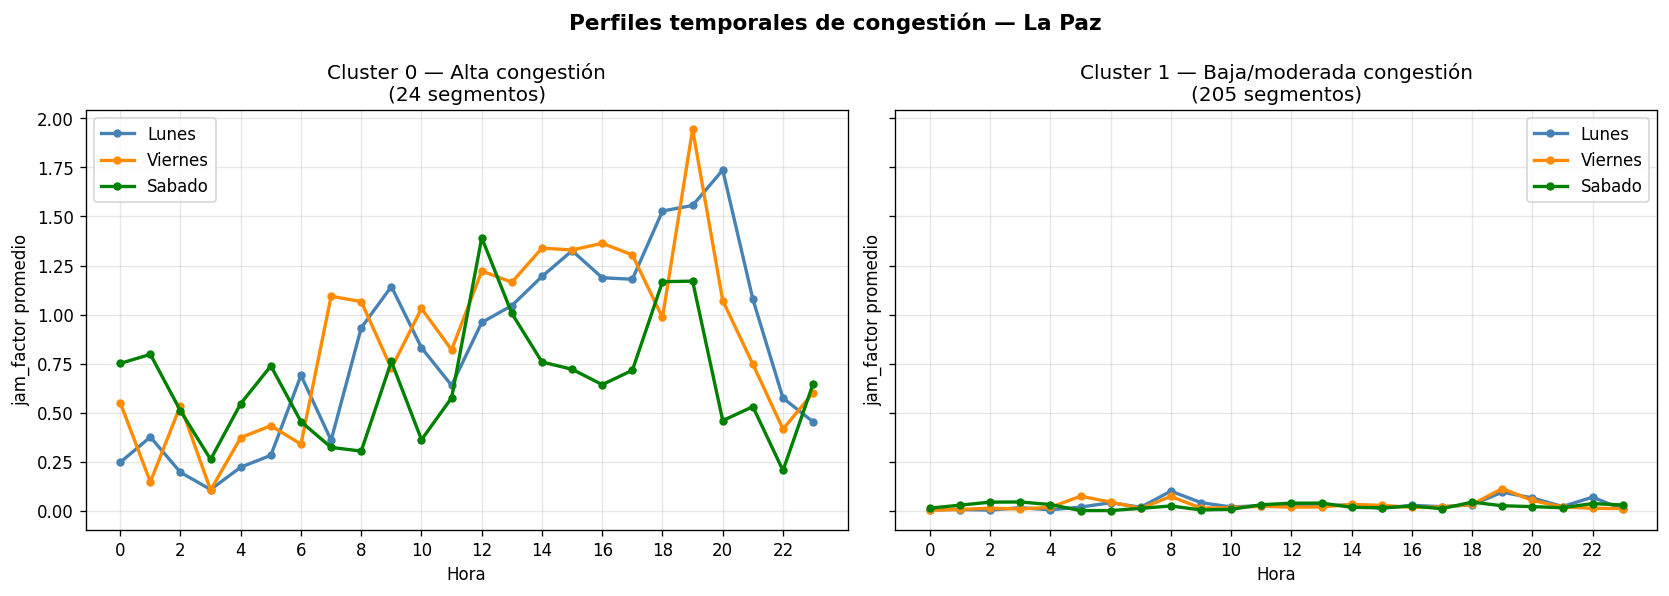
\includegraphics[width=0.90\textwidth]{img/perfiles_24h.png}
  \caption{Curvas de congestión por hora del día para los dos clusters,
           en los distintos días recolectados.
           El cluster de alta congestión muestra picos pronunciados a las
           8 h y 17 h; el de baja congestión se mantiene plano.}
  \label{fig:perfiles_24h}
\end{figure}

\subsection{Limitaciones}

\begin{enumerate}
  \item \textbf{Muestra.} 250 de $\sim$37\,100 segmentos; algunas calles
    importantes pueden no estar representadas.
  \item \textbf{Datos históricos de Google.} Estimaciones basadas en datos
    anónimos; pueden diferir en eventos especiales (feriados, bloqueos).
  \item \textbf{Días estimados.} Martes, jueves y especialmente domingo
    son síntesis estadísticas; no deben usarse para decisiones críticas.
  \item \textbf{Estacionalidad.} Los datos corresponden a un período
    acotado de 2024--2025; no capturan variaciones estacionales.
\end{enumerate}

%=================================================================
\section{Conclusiones}
%=================================================================

Este proyecto demuestra que el aprendizaje no supervisado permite extraer
conocimiento valioso sobre el comportamiento del tráfico urbano
\emph{sin necesidad de datos etiquetados ni expertos previos}.

\medskip

La combinación de técnicas resultó más rica que cualquier método aislado:
\begin{itemize}[noitemsep]
  \item \textbf{PCA} redujo el ruido y comprimió 96 dimensiones a 13,
    preservando el 86--96\% de la información.
  \item \textbf{UMAP} hizo visible la separación entre grupos en 2D.
  \item \textbf{DBSCAN} identificó vecindades geográficas sin asumir
    formas de cluster ni requerir $k$.
  \item \textbf{K-Means} segmentó los patrones temporales en grupos
    semánticamente interpretables.
  \item \textbf{NMF + PCHIP} completó la semana preservando la
    no-negatividad del jam\_factor y cuantificando la incertidumbre.
\end{itemize}

\medskip

El resultado práctico —el dashboard interactivo— pone esta información
al alcance de cualquier ciudadano o gestor de movilidad,
con etiquetas claras sobre la fiabilidad de cada dato.

\paragraph{Hallazgos sobre La Paz y El Alto.}
La congestión severa en La Paz es \textbf{estructural}: el 10{,}8\,\% de
arterias monitoreadas concentra los patrones de alta congestión, ubicadas
principalmente en el centro histórico y accesos a la autopista.
Intervenciones puntuales en esas arterias tendrían mayor impacto que
medidas de alcance general en toda la red.

El Alto exhibe un comportamiento más homogéneo (96{,}1\,\% de varianza
PCA en 13 dimensiones), con solo el 4{,}0\,\% de segmentos de alta
congestión, todos concentrados en La Ceja: el nodo de transferencia entre
ambas ciudades.
Mejorar la fluidez en La Ceja reduciría la congestión de manera
desproporcionada respecto a cualquier otra intervención en El Alto.

Los modelos no supervisados confirman que la diferencia de congestión
entre barrios de La Paz no es un continuo sino una \textbf{dicotomía}:
hay calles que casi siempre se congestión y calles que casi nunca lo hacen.
Esta estructura binaria emergió sin haber etiquetado previamente ningún
segmento como ``congestionado'' o ``libre'', lo que valida la capacidad
del aprendizaje no supervisado para descubrir patrones genuinos en datos
de tráfico real.

\paragraph{Trabajo futuro.}
Con datos históricos de más días y semanas sería posible aplicar
modelos de series temporales (LSTM, Prophet) para predicción en tiempo real,
e incorporar datos de precipitación o eventos para modelos de impacto vial.

%=================================================================
\appendix
\section{Dependencias del proyecto}
%=================================================================

\begin{lstlisting}[language=bash, caption={requirements.txt resumido.},
    keywordstyle=\color{azulAS}]
flask>=3.0
pandas>=2.0
numpy>=1.26
scikit-learn>=1.4
scipy>=1.12
umap-learn>=0.5
folium>=0.16
osmnx>=1.9
plotly>=5.20
matplotlib>=3.8
\end{lstlisting}

\section{Estructura de archivos}

\begin{lstlisting}[language=bash, caption={Árbol de directorios del proyecto.},
    keywordstyle=\color{azulAS}]
lapaz_traffic/
  data/
    raw/
      sample_segments.csv            # 250 segmentos La Paz
      sample_segments_el_alto.csv    # 250 segmentos El Alto
      traffic_lunes_00.csv ...       # datos recolectados
      el_alto/traffic_*.csv
    processed/
      feature_matrix.csv             # 250 x 168
      feature_matrix_el_alto.csv     # 250 x 168
      segments_clustered.csv         # 500 filas con clusters
      synthetic_days_metadata.csv    # confianza por dia
  notebooks/
    01_red_vial.ipynb
    02_recoleccion.ipynb
    03_preprocesamiento.ipynb
    04_reduccion_dimensionalidad.ipynb
    05_clustering.ipynb
    06_visualizacion.ipynb
  scripts/
    03_rebuild_features.py
    04_rebuild_clustering.py
    05_predict_missing_days.py
  templates/
    index.html
    map.html
  dashboard.py
  informe/
    informe.tex
    informe.pdf
    gen_map.py
    img/
      red_vial.png
      perfiles_raw.png
      preprocesamiento.png
      pca_varianza.png
      umap_proyeccion.png
      mapa_clusters.png
      kmeans_codo.png
      perfiles_clusters.png
      perfiles_24h.png
\end{lstlisting}

\end{document}
